
\documentclass[12pt]{article}
\usepackage{fullpage,amsmath,amssymb,graphicx}

\usepackage{setspace}
\spacing{1}

\usepackage{textpos}
\usepackage{tikz}
\usepackage{pgf}
\usepackage{amssymb}
\usepackage{enumerate}
\usepackage{xcolor}
\usepackage{graphicx}
\usepackage{subcaption}
\usepackage{tabularx}
\usepackage{colortbl}
\usepackage{multicol}
\usepackage{longtable}
\usepackage{hyperref}
\usepackage{comment}
\usepackage{listings}

\lstdefinestyle{mystyle}{
    backgroundcolor=\color{lightgray},   
    commentstyle=\color{green},
    keywordstyle=\color{blue},
    numberstyle=\tiny\color{gray},
    stringstyle=\color{red},
    basicstyle=\ttfamily\footnotesize,
    breakatwhitespace=false,         
    breaklines=true,                 
    captionpos=b,                    
    keepspaces=true,                 
    numbers=left,                    
    numbersep=5pt,                  
    showspaces=false,                
    showstringspaces=false,
    showtabs=false,                  
    tabsize=2
}
\lstset{style=mystyle}


\definecolor{encabezado}{rgb}{0.74, 0.83, 0.9}

\begin{document}

\hfill\\
\rule{\textwidth}{1.5pt}

\begin{minipage}[t]{85mm}
  \begin{tabular}{l}
    \textbf{\large Instituto Tecnológico de Costa Rica} \\  
    \textbf{Escuela de Ingeniería Electrónica} \\
    \textbf{Trabajo Final de Graduación} \\
    \textbf{Proyecto:} Método basado en aprendizaje reforzado \\para el control automático de una planta no lineal. \\
    \textbf{Estudiante:} Oscar Andrés Rojas Fonseca \hspace{3cm}\rule{4.5cm}{1.5pt}\\
    I Semestre 2024 \hspace{8.5cm}\textbf{Firma del asesor}
  \end{tabular}
\end{minipage}
\hfill\\
\rule{\textwidth}{1.5pt}


\section*{Bitácora de trabajo}

%\begin{table}[h]
\begin{minipage}[h]{\textwidth}
	\centering
	\begin{tabularx}{\textwidth}{|p{2cm}|X|X|p{2cm}|} 
		\hline
		\rowcolor{encabezado}
		\textbf{Fecha} & 
		\textbf{Actividad} & 
		\textbf{Anotaciones} & 
		\textbf{Horas dedicadas} \\ \hline
		% ***************************************************************
	 	08/05/2024 & 
	 	$\mathbf{1}.$ Reunión de seguimiento con el asesor del proyecto. & 
	 	$a)$ Revisión de avance y errores de forma. \newline
	 	$b)$ Replanteamiento de la función de recompensas. Cambio a $np.min()$ para los parámetros y cambio en recompensa de duración. \newline & 
	 	2 horas \\
        % ***************************************************************
	 	08/05/2024 & 
	 	$\mathbf{2}.$ Entrenamiento del modelo $PPO$ con nueva definición de $self.theta\_good$. & 
	 	$a)$ Se probó con hasta $1M$ de steps, mal resultado. \newline & 
	 	6 horas \\
		% ***************************************************************
	 	09/05/2024 & 
	 	$\mathbf{3}.$ Entrenamiento del modelo $PPO$ con nueva definición de $self.theta\_good$. & 
	 	$a)$ La falta de mejora en el resultado indicó un error en la valoración (función $evaluate()$), en revisión. \newline
	 	$b)$ Ajuste en parámetro $self.theta\_good$ por diferencia de escala. \newline & 
	 	6 horas \\
        % ***************************************************************
	 	09/05/2024 & 
	 	$\mathbf{4}.$ Entrenamiento del modelo $DQN$ discreto con nueva definición de $self.theta\_good$. & 
	 	$a)$ Prueba de nueva función de recompensas con el código $DQN$ discreto. \newline
	 	$b)$ Resultados insatisfactorios demostraron la necesidad de disminuir el rango de trabajo del \textit{action space}, resolución de la discretización. \newline & 
	 	6 horas \\
		% ***************************************************************

	 	\hline
	\end{tabularx}
\end{minipage}	 	
	 	
	 	% ***************************************************************
\hfill\\
\begin{minipage}[h]{\textwidth}
	\centering
	\begin{tabularx}{\textwidth}{|p{2cm}|X|X|p{2cm}|} 
		\hline		

            % ***************************************************************
		  10/05/2024 & 
	 	$\mathbf{5}.$ Pruebas de entrenamiento del modelo $PPO$ y ajustes al $torch.clamp()$ al \textit{action space}. &
	 	$a)$ Se determina que el entrenamiento y acciones del modelo imitador del $PAMH$ entrenó con acciones suficientes de $PWM$ en el rango $[0.0, 0.25]$. Se disminuye el rango para el modelo controlador. \newline
	 	$b)$ Primera versión del ajuste de las distribuciones con la señal del $OU\_process()$ no mostró resultado satisfactorio. \newline & 
	 	10 horas \\
	 	% ***************************************************************
	 	13/05/2024 & 
	 	$\mathbf{6}.$ Entrenamientos del modelo $PPO$ y ajustes a función de recompensas. &
	 	$a)$ Los resultados mostraban tendencia al aumento de velocidad angular, por lo que se aumentó el peso de la velocidad en el reward con buen  resultado. \newline
            $b)$ Se probó mudar los entrenamientos a la plataforma $Google\, Colaboratory$. Disminución de los tiempos en aproximadamente $50\%$ \newline &
	 	6 horas \\
	 	% ***************************************************************
	 	14/05/2024 & 
	 	$\mathbf{7}.$ Entrenamientos del modelo $PPO$ y ajustes a función de recompensas. &
	 	$a)$ Se continuó con los ajustes de $self.theta\_good$ para mejorar su escala respecto a los otros parámetros. Resultados insatisfactorios. \newline
            $b)$ Pruebas de entrenamientos sin el componente $self.theta\_good$. En ocaciones presenta mejoría. \newline & 
	 	4 horas \\
	 	% ***************************************************************
	 	
	 	\hline
		\multicolumn{3}{|r|}{Total de horas de trabajo:} & 40 horas \\ 
	 	\hline                 
	\end{tabularx}
\end{minipage}


% *****************************************************************************
% *****************************************************************************
% *****************************************************************************
\newpage

\section*{Contenidos de actividades}

%\begin{figure}[h!]
%	\centering
%	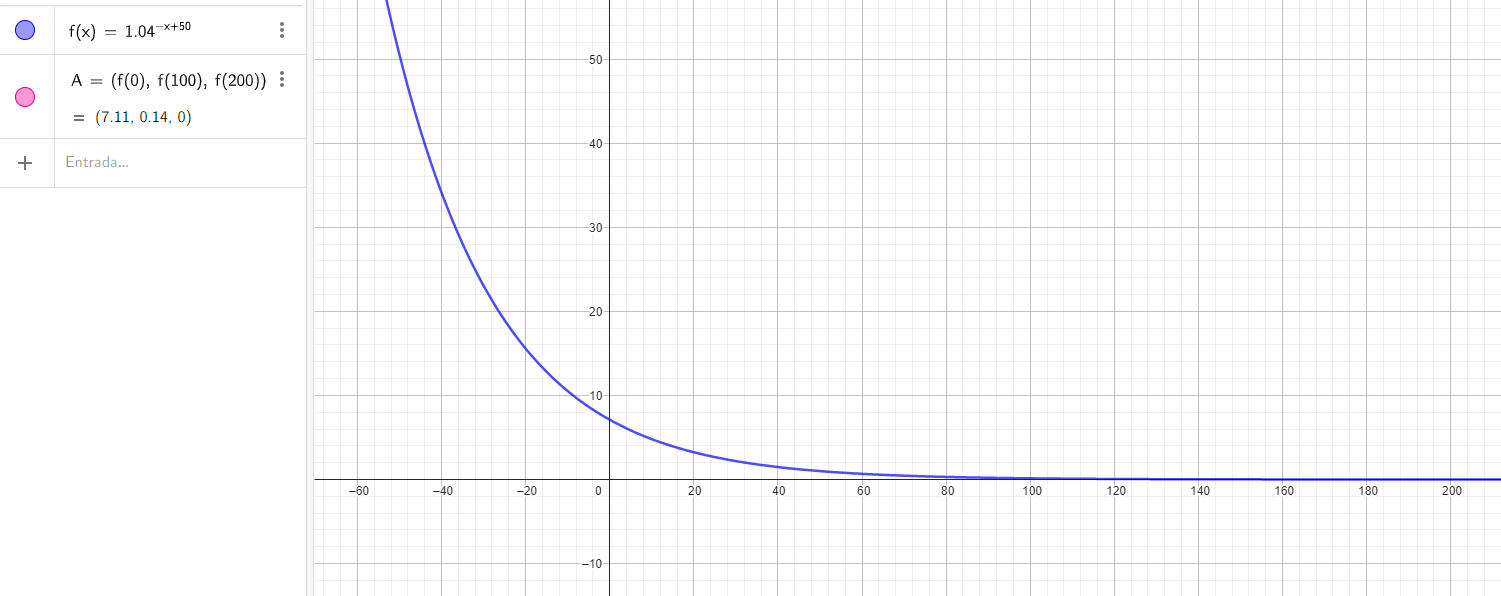
\includegraphics[scale=0.26]{Fig/Captura_funcion.png}
%	\caption{Función utilizada para castigar la corta duración del episodio.}
%	\label{fig:funcion}
%\end{figure}

Luego de numerosas pruebas con la definición de la función de recompensas; ajustes de pesos en los parámetros $theta\_error\_cost$, $velocity\_cost$, $extra\_cost$ y $self.theta\_good$, se llega a la siguiente definición:

\begin{lstlisting}[language=Python, caption=Función de recompensas utilizada]
    def calculate_reward(self, observ, pwm, target_angle): # Todos los valores estan en radianes
        theta = observ[0]
        theta_dot = observ[1]
        
        theta_n = ((theta + np.pi) % (2*np.pi)) - np.pi
        theta_error = np.abs(theta_n - target_angle)
        theta_error_cost = (theta_error ** 2)
        
        velocity_cost = 100 * (theta_dot ** 2)
        
        # 0.1745 rad -> 10 degrees
        # 0.0873 rad -> 5 degrees
        if theta_error <= 0.1745:
            if self.theta_good < 0.0:
                self.theta_good = 0.0
            else:
                self.theta_good += 0.2
        else:
            if self.theta_good > 0.0:
                self.theta_good = 0.0
            else:
                self.theta_good -= 0.2
        if pwm < 0.0 or pwm > 0.25:
            extra_cost = 10 ** np.absolute(pwm - 0.25) - 0.25
        else:
            extra_cost = 0.0
        
        reward_n = np.min([-velocity_cost, -theta_error_cost, -extra_cost]) + self.theta_good
        return reward_n.item()
\end{lstlisting}

Con ayuda del asesor del proyecto se encontró una fuente con amplios detalles respecto al funcionamiento del algoritmo $PPO$ \cite{37PPO}, donde se detallan enfoques respecto a diferentes tipos de modelos a controlar, discretos o continuos, y se muestran sus resultados respectivos, lo cual ayuda a reivindicar algunos pasos anteriormente determinados y reconsiderar otros, como el caso de la funcion de recompesas.

\newpage

\section*{Referencias}
\renewcommand\refname{}
\bibliographystyle{IEEEtran}
\bibliography{references}





\end{document}
